\documentclass[a4paper,12pt]{article}
\usepackage[utf8]{inputenc}
\usepackage[T1]{fontenc}
\DeclareUnicodeCharacter{2009}{\,}
\DeclareUnicodeCharacter{2248}{\ensuremath{\approx}}
\usepackage{amsmath, amssymb}
\usepackage{graphicx}
\usepackage{hyperref}
\usepackage{geometry}
\usepackage[style=authoryear]{biblatex}
\usepackage{listings}
\usepackage{eso-pic}
\usepackage{graphicx}
\usepackage{xcolor}
\usepackage{hyperref}
\usepackage{pgfplots}
\usepackage{float}
\pgfplotsset{compat=1.18}
\lstdefinelanguage{json}{
    basicstyle=\ttfamily\small,
    numbers=left,
    numberstyle=\tiny,
    stepnumber=1,
    numbersep=5pt,
    showstringspaces=false,
    breaklines=true,
    frame=lines,
    backgroundcolor=\color{gray!10},
    literate=
     *{0}{{{\color{blue}0}}}{1}
      {1}{{{\color{blue}1}}}{1}
      {2}{{{\color{blue}2}}}{1}
      {3}{{{\color{blue}3}}}{1}
      {4}{{{\color{blue}4}}}{1}
      {5}{{{\color{blue}5}}}{1}
      {6}{{{\color{blue}6}}}{1}
      {7}{{{\color{blue}7}}}{1}
      {8}{{{\color{blue}8}}}{1}
      {9}{{{\color{blue}9}}}{1},
}

\addbibresource{bibliografia.bib}
\geometry{margin=2.5cm}

\title{%
  \textbf{DollarPunk}\\[1em]
  {\large \textit{ETL-NLP per il monitoraggio del sentiment e il supporto decisionale in finanza comportamentale}}%
}
\author{Alessandro Beninati}
\date{\today}

\begin{document}

\maketitle
\newpage
\section{Motivazione}
 Durante la mia carriera professionale, ho lavorato per tre anni in consulenza informatica
 nel campo dell’ingegneria dati, concentrandomi sull’organizzazione e la gestione di fussi
 dati tramite processi ETL al servizio di alcune delle più grandi aziende italiane. Ho avuto
 la possiblità di vedere coi miei occhi quali dati vengo usati e ho dovuto migrare spesso
 codici che li gestivano da piattaforme on-premises a piattaforme cloud.
 Questa esperienza mi ha permesso di osservare da vicino quanto questi sistemi possano diventare complessi.
Partendo da queste esperienze, ho iniziato a pormi alcune domande: \\\\\textit{In quali casi la tecnologia può essere realmente spinta al limite? }\\\\\textit{In che modo i dati non strutturati, come le news dei media o i posts sui social, possono essere usati per generare valore? }
 \\
\\Con questa proposta di ricerca si intende sviluppare un applicativo che supporti l’utente nel monitoraggio del sentiment digitale relativo a una lista di titoli finanziari.  
\section{Stato dell'arte}
Uno degli studi pionieristici della \textit{sentiment analysis} è quello di \textcite{tetlock2007giving}.\\
In particolare, Tetlock ha quantificato il “pessimismo” degli articoli del Wall Street Journal e trovato che livelli elevati di tono negativo nella stampa anticipano pressioni al ribasso sui prezzi azionari, seguite poi da un ritorno ai fondamentali di mercato.\\
Questo risultato iniziale ha fornito evidenza che il sentiment estratto dai testi – ad esempio il tono pessimista o ottimista delle notizie –  può influenzare il comportamento di mercato.
\subsection{Social media e Sentiment degli Investitori}
Con la diffusione dei social media e delle piattaforme online negli anni 2010, la fonte dei dati sul sentiment si è ampliata. Gli investitori, specialmente retail, hanno iniziato a esprimere opinioni su forum finanziari, Twitter e blog, fornendo un flusso di testo ricco di informazioni sul sentiment di mercato in tempo reale. \\ 
La letteratura in questo periodo ha esaminato in che misura il sentiment influenzi i rendimenti azionari, spesso in contrasto con la teoria finanziaria tradizionale che esclude fattori emotivi. \textcite{mcgurk2020stock} mostrano chiaramente questo cambio di paradigma: analizzando i post sui social media, questi autori costruiscono una misura quantitativa del sentiment degli investitori e trovano che tale misura ha un effetto positivo e significativo sui rendimenti anomali delle azioni.

Un caso emblematico che ha catalizzato l’interesse sull’analisi del sentiment è la pandemia di COVID-19. \textcite{duan2021covid} \textit{et alter} sviluppano ad esempio indici di sentiment legati al COVID-19 usando milioni di testi provenienti sia dai media ufficiali che dai social in Cina.
\subsection{L'avvento dei modelli Transformer e di FinBERT}

Alla fine degli anni 2010, l’introduzione di BERT (\textcite{devlin2018bert}) ha rivoluzionato l’NLP anche in ambito finanziario, grazie a rappresentazioni linguistiche contestuali di alta qualità. Tuttavia, l’adattamento al linguaggio tecnico della finanza ha richiesto modelli specializzati. FinBERT, proposto da \textcite{araci2019finbert}, è stato il primo modello pre-addestrato su testi finanziari e poi fine-tunato per il sentiment analysis, superando di circa 15 punti percentuali i metodi precedenti su dataset come \textit{Financial PhraseBank}.

Versioni successive come quella di \textcite{huang2022finbert}, addestrata su grandi corpora finanziari, hanno raggiunto fino all’89,7\% di accuratezza nel rilevare frasi negative, migliorando la comprensione delle sfumature linguistiche rispetto ai modelli generici.

FinBERT è oggi uno standard per task NLP finanziari: analisi del tono nei report, classificazione di notizie, estrazione di informazioni da bilanci. \textcite{gu2024finbert} mostrano che un modello FinBERT+LSTM migliora la previsione dei trend azionari rispetto a LSTM tradizionali, evidenziando il valore della specializzazione di dominio.

Infine, l’emergere di benchmark specifici (es. FiQA, Financial PhraseBank) ha supportato valutazioni comparative, mentre estensioni recenti si concentrano su analisi a livello di entità \textcite{tang-etal-2023-finentity}.

\subsection{Modelli di Linguaggio Generali vs. Specifici in Finanza}

Nel 2022-2023, l’attenzione si è spostata sui LLM generici come ChatGPT (GPT-3.5/4), capaci di interpretare testi finanziari nonostante l’assenza di addestramento settoriale. \textcite{lopezlira2024chatgptforecaststockprice} mostrano che ChatGPT può prevedere la direzione dei prezzi azionari basandosi sui titoli delle notizie. Anche in modalità zero-shot, modelli come GPT-3.5/4 riescono a svolgere sentiment analysis su documenti finanziari pur con limiti su contesti specialistici o eventi recenti. (\textcite{bdcc8110143})

Questi risultati hanno spinto verso LLM specializzati. BloombergGPT \textcite{wu2023bloomberggptlargelanguagemodel}, con 50 miliardi di parametri e un corpus di 363 miliardi di token finanziari, è il primo LLM su larga scala dedicato alla finanza, con maggiore precisione su prompt settoriali grazie alla sua conoscenza approfondita del dominio.

In parallelo, il progetto open-source FinGPT \textcite{yang2023fingptopensourcefinanciallarge} punta a rendere i LLM finanziari accessibili, attraverso fine-tuning di modelli open-source su dati finanziari pubblici. Con un approccio data-centric, FinGPT abilita analisi di sentiment, generazione automatica di report e sviluppo low-code, pur operando con risorse più contenute rispetto ai modelli proprietari.

\subsection{Sviluppi Recenti e Tendenze dal 2024 in poi}

Nonostante i progressi, restano sfide aperte nell’NLP per il sentiment finanziario. \textcite{bdcc8110143} mostrano che un semplice modello di regressione logistica ha superato FinBERT e GPT-4 in accuratezza, segnalando che maggiore complessità non implica sempre migliori performance.

Nuove metriche ampliano le prospettive: \textcite{cao2025hypeindexnlpdrivenmeasure} propongono l’Hype Index, che misura l’attenzione mediatica anziché il tono. Analizzando l’S\&P 100, dimostrano che un picco di copertura può anticipare volatilità e movimenti di mercato, sottolineando il valore dell’“intensità” informativa come fattore predittivo.

In sintesi, dal 2000 al 2025 l’evoluzione dei modelli NLP è passata da analisi semplici a LLM avanzati. Le tendenze attuali puntano su AI spiegabile, modelli integrati in flussi real-time e analisi che considerano non solo sentiment, ma anche attenzione, emozioni e dinamiche testuali complesse, rendendo il campo sempre più ricco e maturo.

\section{Descrizione del progetto}
\subsection{Strumenti di sviluppo, versioning e hosting}

Il progetto adotta un approccio rapido e sperimentale, supportato da strumenti AI per refactoring, debugging e generazione di codice, sotto supervisione umana. Il codice sarà gestito via GitHub con checkpoint strategici.

Si utilizzeranno Python, Rust o JavaScript secondo i moduli, con architettura containerizzata (es. Docker) per garantire portabilità. L’hosting server/API sarà valutato tra PaaS e VPS, bilanciando costi e controllo. Per calcoli intensivi o training si ricorrerà a servizi cloud come Databricks o RunPod.

L’impostazione resta flessibile, pronta a correzioni in corso d’opera. Una demo è disponibile a:
\href{https://unime01-d9a3b5f15d3b.herokuapp.com/}{\textit{\textbf{Financial News Collection Demo}}}
\subsection{Raccolta Dati}

La previsione dei movimenti di mercato richiede l’acquisizione di grandi volumi di dati testuali da fonti eterogenee:

\begin{itemize}
    \item \textbf{Fonti finanziarie:} Bloomberg, Reuters, WSJ, Yahoo Finance, ANSA, Il Sole 24 Ore, Investing.com, ecc.
    \item \textbf{Social media e community:} Twitter, Reddit (\textit{r/investing}, \textit{r/wallstreetbets}), LinkedIn, Telegram, YouTube.
    \item \textbf{Motori di ricerca:} SerpApi, \texttt{duckduckgo-search}, \texttt{ddgs}.
    \item \textbf{Temi di interesse:} sentiment finanziario, trend macroeconomici, eventi geopolitici, earning reports, indicatori ESG, criptovalute.
\end{itemize}

L’acquisizione avverrà via scraping (es. libreria \texttt{newspaper}) o tramite API quando possibile. Su Reddit, sarà rilevante raccogliere anche commenti, upvotes e metriche social. Per tutti i canali, sarà definita una strategia per strutturare e contestualizzare i dati in modo coerente.

\subsection{Analisi dati testuali}
Una volta raccolti dati testuali in quantità adeguata, sarà utile sviluppare una funzione che elabori il testo (sia una news o un post) e restituisca un array JSON con le informazioni principali vale a dire: ticker menzionati, \emph{relevance score} e \emph{sentiment score}.

\vspace{0.3cm}
\newpage
\paragraph{Esempio di output atteso:}

\begin{lstlisting}[language=json]
[
{
"title": "If You Invested $1,000 In Lululemon Stock In 2013, Here's How Much You'd Have Now",
"url": "https://www.fool.com/investing/2023/04/30/if-you-invested-1000-in-lululemon-stock-in-2013-he/",
"source": "Motley Fool",
"time_published": "2023-04-30T13:34:00",
"stocks_mentioned": ["LULU", "NKE"],
"ticker_sentiments": [
{
"ticker": "LULU",
"relevance_score": 0.11,
"sentiment_score": 0.12,
"sentiment": "Neutral"
},
{
"ticker": "NKE",
"relevance_score": 0.27,
"sentiment_score": 0.22,
"sentiment": "Somewhat-Bullish"
}
]
}
]
\end{lstlisting}

\vspace{0.5cm}

In seguito verranno presentate e valutate diverse soluzioni per identificare e calcolare in modo affidabile i tre campi (\textit{tickers}, \textit{relevance score}, \textit{sentiment score}). Considerata la natura estremamente dinamica e in continua evoluzione del settore NLP applicato alla finanza, nulla esclude che possano emergere approcci o strumenti più efficaci anche nel breve termine, che potranno essere adottati se ritenuti vantaggiosi.

\subsubsection{Tickers}

Per associare un testo al giusto ticker, è utile combinare più segnali: il contesto della raccolta (es. query mirate come "Apple stock"), tecniche di Named Entity Recognition (es. "Apple Inc."), pattern matching (es. \verb|$AAPL|, \verb|(NASDAQ:AAPL)|) e dizionari che mappano nomi aziendali ai ticker.

Un sistema robusto integra queste fonti assegnando un \emph{confidence score}: alto (0.9–1.0) per citazioni dirette o query esplicite, medio (0.6–0.8) per nomi aziendali, più basso per riferimenti indiretti. Questo riduce ambiguità e migliora la precisione nel collegare testo e titolo azionario.

\subsubsection{Relevance score}

Il \textit{relevance score} misura quanto un ticker è centrale in un testo. Un metodo semplice consiste nel contare le occorrenze e normalizzarle per lunghezza o numero totale di ticker.

Approcci più avanzati includono l’uso dei pesi di attenzione nei modelli Transformer, reinterpretati come indicatori di rilevanza \textcite{delcorro2020relevance}, e sistemi commerciali come RavenPack, che valutano frequenza, posizione e ruolo semantico. Il framework News-to-Numbers (Stanford NLP, 2023) assegna punteggi 0–100 a coppie ticker–headline usando LLM \parencite{stanford2023newstonumbers}.

In sintesi, il conteggio base è utile per prototipi, ma applicazioni professionali richiedono metodi più contestuali e automatizzati.

\subsubsection{Sentiment score}

Il \textit{sentiment score} quantifica il tono associato a un ticker in un testo, mappando le polarità (positiva, negativa, neutra) su scale continue (es. –1 a +1), tramite modelli come FinBERT o LLM specializzati.

Per maggiore precisione, si adotta il sentiment a livello di entità (ticker–frase) \parencite{tang-etal-2023-finentity}, come fanno anche sistemi commerciali (Refinitiv, Bloomberg) o open-source (FinGPT \parencite{yang2023fingptopensourcefinanciallarge}). 

In alternativa, modelli zero-shot come GPT-4 possono generare punteggi continui (es. 0–100) via prompt, senza training specifico \parencite{bdcc8110143}, rendendoli utili per pipeline automatizzate e flessibili.

\subsubsection{Fine tuning}

Il fine-tuning di un LLM open source consente di ottenere un modello che, dato un testo, restituisce direttamente un oggetto strutturato con \textit{ticker}, \textit{relevance score} e \textit{sentiment score}. Questo approccio unifica la pipeline ed evita moduli separati, sfruttando la generalizzazione del modello pre-addestrato.


Modelli come \textit{FinBERT} \parencite{araci2019finbert} o \textit{Mixtral}, così come LLM open-source adattabili (es. \textit{FinGPT} \parencite{yang2023fingptopensourcefinanciallarge}), possono essere affinati con dati finanziari annotati. A tal fine, è cruciale disporre di un dataset ampio con etichette a livello di entità (ticker-level sentiment), come quelli forniti da challenge pubbliche \parencite{maia201818} o aggregabili tramite API di notizie come Alpha Vantage.

L’addestramento può essere eseguito su infrastrutture cloud dotate di GPU, offerte da servizi come RunPod, Lambda Labs o Google Cloud. Questo consente di bilanciare costi e prestazioni in modo flessibile \parencite{li2020cloudgpu}.
\subsubsection{Retrieval-Augmented Generation (RAG)}

RAG unisce LLM (es. GPT-4, Mixtral) a un modulo di recupero documentale: il modello genera risposte basate su contesto estratto in tempo reale da un indice vettoriale (es. notizie o headlines finanziarie).

L’input può essere un prompt standardizzato (“Estrai ticker, sentiment score e relevance score”), e il modello produce direttamente un JSON strutturato, senza fine-tuning. Il sistema è aggiornabile modificando i documenti indicizzati \parencite{lewis2020retrieval}.

Strumenti come FAISS e LangChain abilitano una pipeline scalabile e flessibile, come dimostrato da progetti come FinGPT-RAG \parencite{gudibande2023false, yang2023fingptopensourcefinanciallarge}.

\subsubsection{Sintesi}

Disponendo di un dataset etichettato (sentiment per ticker), si possono seguire varie strategie:

\begin{itemize}
  \item \textbf{Fine tuning di FinBERT}: usando GPU (e.g. RunPod), si perfeziona FinBERT affinché generi direttamente JSON con sentiment score per ticker, sfruttando l’apprendimento supervisionato.
  \item \textbf{Fine tuning di LLM open-source generici}: modelli come Mixtral o FinGPT si adattano tramite dataset etichettati, richiedendo anch’essi GPU performanti.
  \item \textbf{Approccio RAG}: se le risorse GPU sono limitate, si indicizza il dataset e si usa un LLM con retrieval (e.g. GPT-4, Mixtral) per generare JSON dal contesto recuperato, evitando il fine-tuning (vedi Lewis et al. 2020).
\end{itemize}

Se non c’è un dataset già annotato:

\begin{itemize}
  \item \textbf{Modello di base con FinBERT}: applicazione zero-shot su frasi per generare sentiment iniziale.
  \item \textbf{GPT-4 via API}: può produrre JSON strutturati, ma su larga scala può risultare costoso.
  \item \textbf{Costruzione manuale del dataset}: si annotano manualmente esempi, utili per successivo fine-tuning anche con risorse limitate.
\end{itemize}
\subsection{Decay temporale (solo sul relevance)}

Una volta calcolati \textit{tickers}, \textit{sentiment} e \textit{relevance} è utile distribuirli nel tempo per ottenere una visione aggregata su base giornaliera.  
Per farlo, proponiamo di applicare un decadimento temporale al solo \textit{relevance score}: il sentiment resta invariato, ma viene ponderato in base alla rilevanza residua della notizia nei giorni successivi alla pubblicazione.

L’obiettivo è costruire, per ogni giorno, una misura sintetica del sentiment attivo nel mercato, che tenga conto del fatto che l’impatto informativo di una news tende a ridursi con il tempo.

\subsubsection*{Esempio}

Nella tabella seguente, il relevance score viene attenuato giorno per giorno, mentre il sentiment associato rimane fisso:

\begin{center}
\renewcommand{\arraystretch}{1.4}
\begin{tabular}{|c|c|c|c|}
\hline
\textbf{News \#} & \textbf{Giorno 0} & \textbf{Giorno 1} & \textbf{Giorno 2} \\
\hline
1 & S=1.000,\ R=0.800 & S=1.000,\ R=0.593 & S=1.000,\ R=0.442 \\
2 & ---               & S=0.900,\ R=0.700 & S=0.900,\ R=0.518 \\
3 & S=0.750,\ R=0.600 & S=0.750,\ R=0.444 & S=0.750,\ R=0.329 \\
\hline
\textbf{Media ponderata} & $\approx$0.892 & $\approx$0.716 & $\approx$0.697 \\
\hline
\end{tabular}
\end{center}
Il relevance viene attenuato con una funzione esponenziale:

\[
R_{i,d} = R_{i,0} \cdot e^{-\lambda \Delta t}, \quad S_{i,d} = S_{i,0}
\]
\begin{figure}[H]
\centering
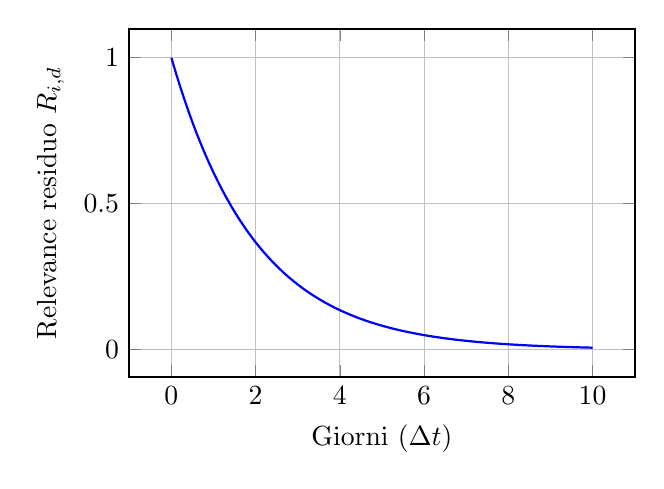
\begin{tikzpicture}
\begin{axis}[
    width=8cm,
    height=6cm,
    xlabel={Giorni ($\Delta t$)},
    ylabel={Relevance residuo $R_{i,d}$},
    grid=major,
    domain=0:10,
    samples=100,
    thick,
]
\addplot[blue] {exp(-0.5*x)};
\end{axis}
\end{tikzpicture}
\caption{Decay esponenziale del relevance score con $\lambda = 0.5$}
\end{figure}

Dove:
\begin{itemize}
  \item $R_{i,0}$ e $S_{i,0}$ sono rispettivamente i valori di relevance e sentiment \textbf{iniziali} della news $i$
  \item $\Delta t$ è il numero di giorni trascorsi dalla pubblicazione
  \item $\lambda$ è un parametro di decay da stimare
\end{itemize}

Per ogni giorno $d$, si calcola la media del sentiment pesata per relevance:

\[
\text{AvgW}_d = \frac{\sum_i \left(S_{i,0} \cdot R_{i,d}\right)}{\sum_i R_{i,d}}
\]

L'approccio è coerente con le logiche adottate da provider come RavenPack, che applicano decay esponenziali al relevance score per modellare la rilevanza informativa nel tempo \parencite{ravenpack_relevance, ravenpack_forex, ravenpack_credit}.
\subsubsection{Sviluppi futuri}

Nel modello presentato in precedenza, il relevance score associato a ciascuna notizia viene attenuato nel tempo secondo un decadimento esponenziale:

\[
R(t) = R_0 \cdot e^{-\lambda t}
\]
Questa funzione è soluzione dell'equazione differenziale ordinaria:

\[
\frac{dR(t)}{dt} = -\lambda R(t)
\]
L'equazione stabilisce una regola che detta la dinamica del decadimento continuo nel tempo, coerente con la logica adottata da vari provider per modellare la perdita di rilevanza delle informazioni.

Tuttavia, questo approccio assume che ogni notizia agisca in modo indipendente. In realtà, molte news trattano argomenti simili, fanno riferimento a eventi collegati o condividono un contesto semantico comune. Trattarle come isolate rischia di ignorare effetti informativi diffusi o correlati.

Un possibile sviluppo futuro consiste quindi nell’estendere il decadimento temporale del relevance score introducendo un termine di diffusione semantica. In altre parole, la rilevanza di una notizia potrebbe non solo decrescere nel tempo, ma anche propagarsi verso altre notizie semanticamente affini.

Questa estensione porta a una generalizzazione dell’equazione di decadimento:

\[
\frac{\partial R(x, t)}{\partial t} = D \nabla^2 R(x, t) - \lambda R(x, t)
\]

Dove:
\begin{itemize}
  \item $R(x, t)$ è il relevance in funzione del tempo $t$ e della posizione $x$ nello spazio semantico (es. embedding del testo),
  \item $D$ è il coefficiente di diffusione semantica,
  \item $\lambda$ è il tasso di decadimento temporale.
\end{itemize}

In questo modello, la rilevanza informativa di una news può diffondersi ad altre notizie simili, modellando una dinamica più realistica del flusso informativo. Il sentiment rimane invariato, ma viene ponderato con $R(x, t)$, che evolve sia nel tempo che nello spazio semantico.

La sfida principale è definire una distanza semantica robusta tra testi, usando embedding, reti di similarità o clustering. In uno spazio semantico coerente, il relevance score può propagarsi tramite metodi numerici o grafi, abilitando applicazioni in risk monitoring, segnali di portafoglio ed eventi informativi.

Ciò permette di concepire il relevance non come punteggio statico, ma come campo dinamico in evoluzione.


\subsubsection{Innovatività e letteratura esistente}

La modellazione del sentiment come campo dinamico che si diffonde tra notizie correlate è ancora poco esplorata. La maggior parte degli studi tratta le news come unità indipendenti o aggrega il sentiment nel tempo.

Alcuni lavori recenti si avvicinano: \textcite{wan2021sentimentdiffusion} mostrano la diffusione del sentiment in reti informative, mentre \textcite{wang2024finin} introducono FININ, che considera interazioni semantiche tra notizie per predire il mercato.

L’uso esplicito di un modello a derivate parziali, come un’equazione di diffusione con decadimento, è però inedito in ambito NLP-finance. Questa formulazione continua e interpretabile supera reti discrete e media pesate, aprendo a nuove applicazioni in previsione, strategie di portafoglio e interpretazione dei flussi informativi.
\newpage 
\subsection{Analisi esplorativa: sentiment e prezzo}

Dopo la fase di raccolta e scoring, è essenziale verificare se il sentiment estratto ha davvero un legame con l’andamento dei prezzi. L’analisi esplorativa consente un primo controllo di plausibilità, confrontando l'evoluzione giornaliera del sentiment con le variazioni di mercato.

Un approccio semplice prevede grafici comparativi tra sentiment e prezzo di chiusura, uno scatter plot con variazione percentuale del prezzo, e una misura di correlazione (Pearson o Spearman), anche con ritardi temporali.

Studi precedenti, come \textcite{turn0search0} e \textcite{turn0search1}, hanno trovato correlazioni significative tra il sentiment delle notizie e i prezzi di titoli come Apple, Microsoft e Tesla.

Questa fase è iterativa: se non emergono segnali, si torna a rivedere i dati o il metodo di scoring. Se invece la relazione è anche solo parziale, si può proseguire verso modelli più sofisticati.



\subsubsection{Backtesting operativo semplice}

Il backtesting consiste nel simulare l’applicazione di una strategia su dati storici per valutarne l’efficacia. “Back” indica che si opera retroattivamente: si usano serie storiche di sentiment e prezzi per vedere come avrebbe performato una certa logica decisionale.

Un esempio semplice: si entra long se il sentiment è positivo, si resta fuori (o short) se è negativo o neutro. L’ingresso avviene il giorno successivo al segnale, l’uscita a fine giornata o dopo $n$ giorni.

Si valutano metriche come:
\begin{itemize}
  \item Rendimento cumulato vs. benchmark
  \item Accuratezza delle previsioni
  \item Sharpe ratio semplificato
\end{itemize}

È un primo test operativo a bassa complessità. Se i risultati sono promettenti, si può passare a strategie più avanzate.


\subsubsection{Simulazione del portafoglio}

A questo punto, per rendere il test più realistico, si può estendere la strategia a un contesto multi-ticker. La simulazione definisce capitale iniziale, distribuzione tra titoli, regole di uscita (es. stop-loss) e include i costi per trade. L’obiettivo non è ancora ottimizzare, ma capire se, nel complesso, la strategia regge in condizioni credibili. Se i risultati suggeriscono robustezza, allora la fase successiva — con modelli predittivi come LSTM — può essere intrapresa con maggiore fiducia.

\subsubsection{Integrazione con modelli LSTM}

Alla fine un passo possibile è costruire un modello predittivo che usi insieme dati di prezzo, volumi, indicatori tecnici e sentiment. Diversi studi \parencite{turn0search0, turn0search13, turn0academia22} mostrano che combinare questi segnali in un LSTM migliora la capacità di previsione rispetto a usare solo i prezzi.

Ma cos’è un LSTM? È un tipo di rete neurale che serve per analizzare serie temporali, cioè dati che cambiano nel tempo. Funziona così: per fare una previsione sul giorno “di oggi”, il modello guarda una “finestra” di dati dei giorni precedenti (es. ultimi 5 giorni). In ogni finestra, può vedere per esempio prezzo, volume e sentiment di ogni giorno.

In pratica, l’LSTM impara a riconoscere certi schemi nel passato che anticipano cosa succederà dopo. Aggiungendo il sentiment come informazione extra, il modello può capire meglio certi movimenti di mercato che non dipendono solo dai numeri, ma anche da cosa “si dice in giro”.

\newpage
\printbibliography
\section{Aknowledgments}
Ringrazio: \\
    ME per aver reagito. \\
    Mia madre per essere affettuosa.\\
    Mio padre per farmi pescare.\\
    Pippo e Massimo per le colazioni pre accensione.\\
    Armando per aver comprato il dominio \\
    Barbara per avermi parlato.\\
    Nonio per recuperarmi dalla merda. \\
    t4v/acn per avermi supportato emotivamente.\\
\\
\\
Gabriele per stare alti.\\
\end{document}
